\documentclass{article}
\usepackage[utf8]{inputenc}

\title{Répartition des projets industriels de fin d'études}
\author{LECLER Hugo \\ FAIZA Mohamed Iheb \\ GRANEL Joris}
\date{11/10/17}

\usepackage{graphicx}

\begin{document}

\maketitle

\section{Objectif}
Le but du projet est de donner une méthode de création des groupes et de répartition des projets, qui soit équitable, satisfaisante, stable, non manipulable et implémentable.

\section{Modélisation}

\subsection{Définition : Méthode d'attribution des groupes}
Une méthode d'attribution des groupes est un outil permettant de passer d'un ensemble de données non ordonnées à un ensemble ordonné d'éléments afin de résoudre un problème.

\subsection{Données du problème}
Soit :
\begin{itemize}
  \item P = {projet1, … , projetm} l’ensemble des projets avec m le nombre total de projets tel que m≤18.
  \item E = {élève1, … , élèven} l’ensemble des étudiants avec 2 < n ≤ 3m le nombre total des étudiants.
  \item PR = {très bien, bien, assez bien, passable, insuffisant, à rejeter} l’ensemble des préférences.
  \item PREFélève       : 	E →PR    les préférences de l’élève élèvei sur un élève.
  \item PREFprojet      : 	E →PR  les préférences de l’élève élèvei sur un projet.
  \item \textbf{Groupe partiel} : Un groupe partiel est composé de 2 ou 3 élèves.
                Si n ≤ 2m :
                \begin{itemize}
                    \item Si n est impair, on a un groupe partiel de 3 élèves et le reste de 2.
                    \item Sinon, on a que des groupes partiels de 2.
                    \item Sinon, si 2m < n ≤ 3m :
                           → On forme n-2m groupes partiels de 3 et le reste sera des groupes de 2.
                \end{itemize}
                
                \begin{figure}[h!]
                \centering
                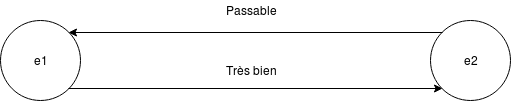
\includegraphics[scale=0.7]{media/groupe_partiel.png}
                \caption{Exemple de groupe partiel}
                \label{fig:univerise}
                \end{figure}
    \item \textbf{Groupe} : Un groupe est composé d'un groupe et d'un projet.
            On décide de modéliser un groupe par un graphe orienté, dont trois ou deux (selon le nombre d'élève) sommets appartiennent à E et le dernier appartient à P. On note l’ensemble des groupes G, par la suite, on distingue deux groupes différents par la notation Gi et Gj, avec i =/= j.
                \begin{figure}[h!]
                    \centering
                    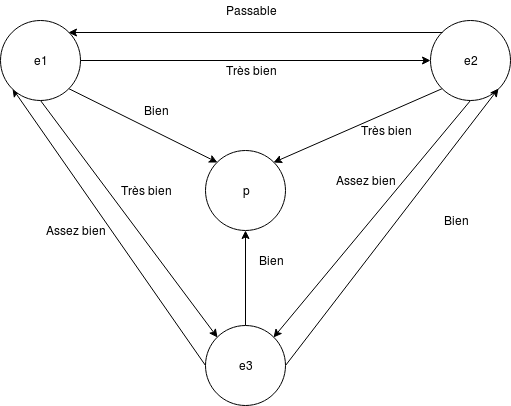
\includegraphics[scale=0.7]{media/groupe.png}
                    \caption{}
                    \label{fig:univerise}
                    \end{figure}
\end{itemize}


\subsection{Relation d’ordre dans l’ensemble des préférences}
On a de manière immédiate que très bien > bien > assez bien > passable > insuffisant > à rejeter. Cette relation est antisymétrique, réflexive et transitive. Ordre lexicographique.

\subsection{Relation d’ordre dans l’ensemble des groupes}
On définit la relation d’ordre dans les groupes par un ordre lexicographique : 
Soit (PRi,1, …, PRi,n) l’ensemble des préférences d’un groupe Gi, trié par ordre croissant.
(PRj,1, …, PRj,m) l’ensemble des préférences d’un deuxième groupe Gj trié par ordre croissant.
Si PRi,1 < PRj,1, alors Gi < Gj.
Si PRi,1 = PRj,1, alors on regarde le 2eme élément de chaque liste.
Si à tout moment on a PRi,k < PRj,k, alors Gi < Gj.
Sinon, si on a n > m et pour tout k ∈ [[1, m]], PRi,k = PRj,k, alors Gi > Gj. 
Sinon, si n = m alors Gi = Gj.
Propriété antisymétrique, réflexive et transitive.  es ce que c’est utile? Le truc c’est es ce que on  l’utilise plus tard


\subsection{Définition des termes du problème}

\textbf{Équitable :} Aucun élève n'est favorisé par la méthode :
Si pour tout (x,y) ∈ E², le seul facteur de l’attribution des groupes est la préférence de chaque élève, aucun autre critère ne doit entrer en compte.

Si deux élèves ont les même préférences, la méthode nous donnera les deux solutions possibles avec les élèves intervertis.
Même chose pour les projets. \par

\textbf{Stable :} Procure une solution meilleure que toutes celles « voisines », c'est à dire que toutes celles en intervertissant deux élèves ou deux projets.
Un groupe est dit stable si en intervertissant un élève ou un projet avec un autre groupe, la satisfaction des deux groupes est inférieure ou égale à celle initiale.
Pour que la méthode soit stable, il faut que tous les groupes soient stable.
Pour tout (élèvex,élèvey) ∈ (E ∩ Gi) x (E ∩ Gj) / (i != j), Gi’ et Gj’ les groupes formés en intervertissant les 2 élèves, Si Gi’ < Gi et Gj’ < Gj, la méthode est stable. \par
\textbf{Non manipulable :}  La meilleure stratégie pour laquelle peut opter un élève est de répondre honnêtement sur ses préférences, c’est à dire que la méthode la plus satisfaisante est également celle où chaque élève n’essaie pas de mentir, soit en étant trop prudent sur ses appréciations, soit en étant trop manichéen. Un élève ne peut alors pas donner une combinaison de préférences élèves - projets qui, sans connaître les préférences de tous les autres élèves, lui assure un groupe précis.
Ex : Un étudiant mettant « À rejeter » à tous sauf 2 élèves et 1 projet n'est pas garanti d'être dans ce groupe précis. \par

\textbf{Satisfaisant :} La méthode est satisfaisante si elle maximise la satisfaction générale des groupes, de la même façon que l’on compare (à l’aide de la relation d’ordre décrite précédemment) des groupes entre eux, on compare des solutions composées de groupe entre elles et on choisit la meilleure.
Soit \[S1 = G^n et S2= G^m/ S1 = (G1,1 , …, G1,n)\] classé à l’aide de la relation d’ordre
				S2 = (G2,1 , …, G2,m) classé par la relation d’ordre
(A finir)
De plus, la méthode est satisfaisante si elle tente de satisfaire le plus grand nombre d’élèves; si un élève est très insatisfait, il sera possible de réduire la satisfaction des autres élèves pour augmenter celle du premier. \par


\textbf{Implémentable :} Il doit être possible d'appliquer la méthode sous forme d'un algorithme qui se termine assez vite pour être utilisé dans le contexte de l’attribution des groupes de projets industriels de fin d’étude. \par



\end{document}
